\section{Mise en place de l'infrastructure}
\subsection{Accès ssh à la raspberry pi}
La raspberry pi a été configurée avec l'adresse IP 192.168.1.2. Il faut configurer l'ordinateur avec une adresse IP 192.168.1.x et le masque réseau 255.255.255.0, cela permet aux deux appareils de communiquer.
\subsubsection{Configuration pour VirtualBox}
Pour partager la connexion dans une machine virtuelle, il faut régler le réseau en \textit{Accès par pont} comme le montre l'image ci-dessous.
\begin{figure}[H]
	\begin{center}
		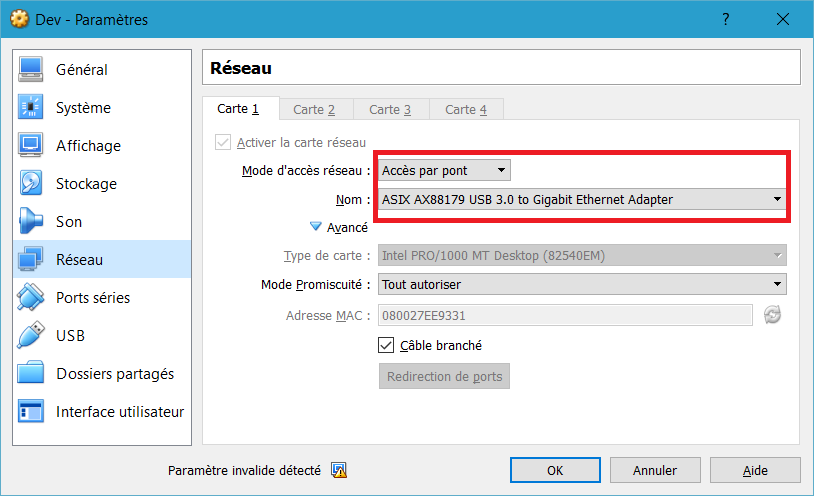
\includegraphics[width=14cm]{img/vmConfig1.png}
		\caption{Configuration de la carte réseau}
		\label{evLinuxConfig1}
	\end{center}
\end{figure}
Il faut également couper la connexion wifi de l'ordinateur, cela lui permettra de se brancher sur la connexion Ethernet.\\
La dernière étape consiste à aller modifier l'adresse IP de la machine virtuelle en changeant les paramètres IPv4. Nous lui avons attribué l'adresse 192.168.1.100.
\begin{figure}[H]
	\begin{center}
		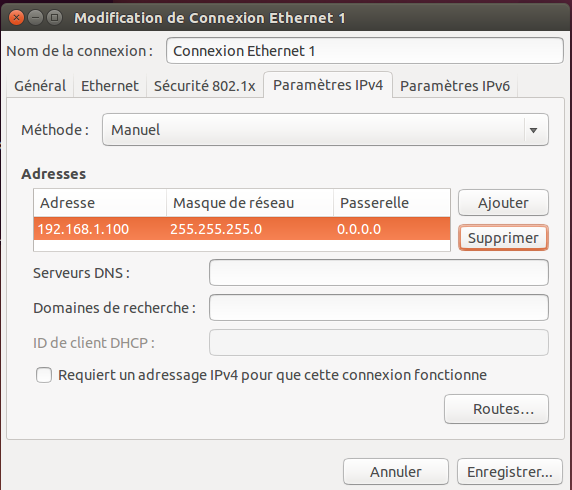
\includegraphics[width=14cm]{img/vmConfig2.png}
		\caption{Changement de l'adresse IP}
		\label{evLinuxConfig2}
	\end{center}
\end{figure}
Il est maitenant possible d'accéder à la raspberry pi par ssh:
\begin{lstlisting}
	$ ssh pi@192.168.1.2
	The authenticity of host '192.168.1.2 (192.168.1.2)' can't be established.
	ECDSA key fingerprint is 80:b2:dc:9d:a5:4e:e7:1a:32:60:11:1c:8b:44:39:0e.
	Are you sure you want to continue connecting (yes/no)? yes
	Warning: Permanently added '192.168.1.2' (ECDSA) to the list of known hosts.
	pi@192.168.1.2's password: 
	...
	pi@raspberrypi:~ $ 
\end{lstlisting}
\subsection{Connexion du capteur}
Pour connecter le capteur à la clé Z-wave, il faut suivre les étapes suivantes:
\begin{enumerate}
	\item Déconnecter le Z-Stick de la Raspberry
	\item Presser le bouton du Z-stick, la LED doit clignoter lentement en bleu
	\item Presser le bouton du capteur
	\item Quand le capteur est inclu/détecter par le Z-Stick, la LED des deux éléments reste figée (vert pour le capteur, bleu pour la clé) quelques instants
	\item Le stick peut ensuite être branché à la Raspberry
\end{enumerate}
\section{Fonctions à implémenter}
Nous nous sommes basés sur la documentation de cette adresse pour implémenter les fonctions. \url{https://python-openzwave.googlecode.com/hg-history/c2d93bd3574e73b828dd86da40d80bbed8c25749/docs/_build/html/index.html}
\subsection{get\_luminance}
\begin{lstlisting}

\end{lstlisting}
\subsection{get\_motion}
\begin{lstlisting}

\end{lstlisting}
\subsection{get\_battery\_level}
\begin{lstlisting}

\end{lstlisting}
\subsection{get\_all\_measures\_sensors}
\begin{lstlisting}

\end{lstlisting}
\subsection{addNode}
\begin{lstlisting}

\end{lstlisting}
\subsection{removeNode}
\begin{lstlisting}

\end{lstlisting}
\subsection{get\_nodes}
\begin{lstlisting}

\end{lstlisting}
\section{REST Client API}
Même si nous n'avions aucune connaissance préalable du REST (discuté lors du premier cours), nous avons tout de même implémenté le client.\\
Nous avons choisi d'utiliser QTCreator et créé une petite application en C++.
\begin{figure}[H]
	\begin{center}
		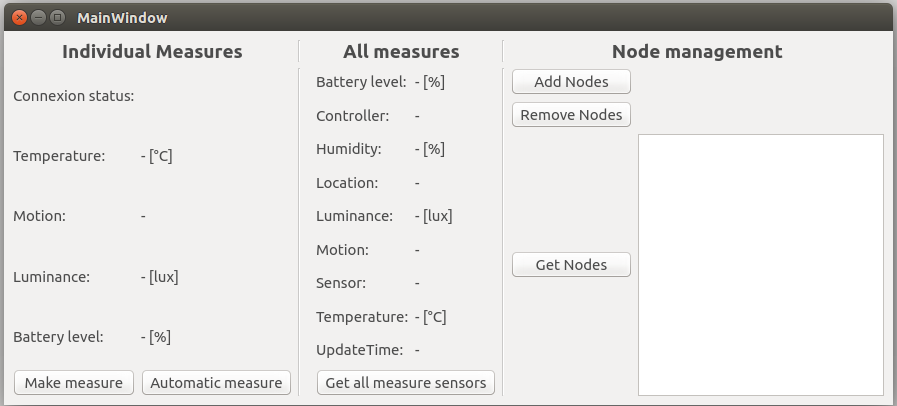
\includegraphics[width=17cm]{img/api.png}
		\caption{Vue par défaut de l'API}
		\label{api}
	\end{center}
\end{figure}
L'API essaie de communiquer avec le nœud  numéro 3. Nous n'avons implémenter la possibilité de changer le numéro.\\
La vue de l'application a été séparée en trois parties distinctes. La première va appeler à la suite les différentes méthodes retournant la température, la luminosité, etc... La partie centrale va appeler la fonction \textit{get\_all\_measures\_sensors}, tandis que la dernière partie permet d'ajouter/supprimer et voir les nœuds du réseau.\\
La première partie possède un champ indiquant si le nœuds répond ou non aux requêtes. Elle contient également un bouton enclenchant le mode automatique, les mesures sont répétées toutes les 10secondes, même si nous avons vu que les valeurs se mettent uniquement à jour chaque 10 minutes.
